%===================================================================================================
%
%===================================================================================================
\chapter{NDTを用いた位置同定}
%---------------------------------------------------------------------------------------------------
\section{概念}
第1章では,様々な位置同定の方法と問題点について述べた.その中でも,本研究ではステレオカメラを用いた3次元計測データと地図データを利用したNDTによる位置同定法について検討する.
NDTとは,Normal Distribution Transformの略語である.文献[1]では,NDTにより生成されるデータとして,ND Voxelと代表平面,および7つの代表点を用いた.また確率的な位置の同定手法としてパーティクルフィルタを用いた.パーティクルフィルタを用いて地図データと計測データとの尤度計算を行い,位置同定する.第2章ではNDTを用いた位置同定について説明し,NDT,パーティクルフィルタの概念について述べた後,実際の位置同定を行うシステムの流れについて述べる.

\newpage
%
%---------------------------------------------------------------------------------------------------
\section{Normal Distribution Transform(NDT)}
NDT(Normal Distributions Transform)とは空間を格子状に分割し,それぞれの格子内に含まれる観測点群の位置に対して分散行列を求め,固有値分解することで得られる分散値による3次元正規分布で空間を表現する手法である.NDTの概念を図{\ref{NDTの概念}}に表す.前述した通り,NDTにより生成されるデータとして,文献[1]ではND ボクセルと代表平面,および7つの代表点を用いている..\par
まず,NDボクセルとはNDTにより得られた正規分布と平均値を与えた一つの3次元格子を言う.ある点$x_{i}$=($x_{i}$,$y_{i}$,$z_{i}$)とすると,どのボクセルに入っているかを座標値を量子化することで求める.次に,求められたボクセルをボクセルkとすると,ボクセルkに入っている$N_{k}$個の点を$x_{k}$(i=0...$M_{k}$-1)とする.このとき,ボクセルkの平均点$m_{k}$と共分散$ \Sigma_{k} $を以下のように求める.\par

\begin{equation}
m_{k}=\cfrac{1}{N_{k}}\sum_{i=0}^{N_{k}-1}x_{ki}
\end{equation}
\begin{equation}
\Sigma_{k}=\cfrac{1}{N_{k}}\sum_{i=0}^{N_{k}-1}(x_{ki}-m_{k})(x_{ki}-m_{k})^t
\end{equation}

%
\begin{figure}[htbp]
  \vspace{-3mm}
  \begin{center}
   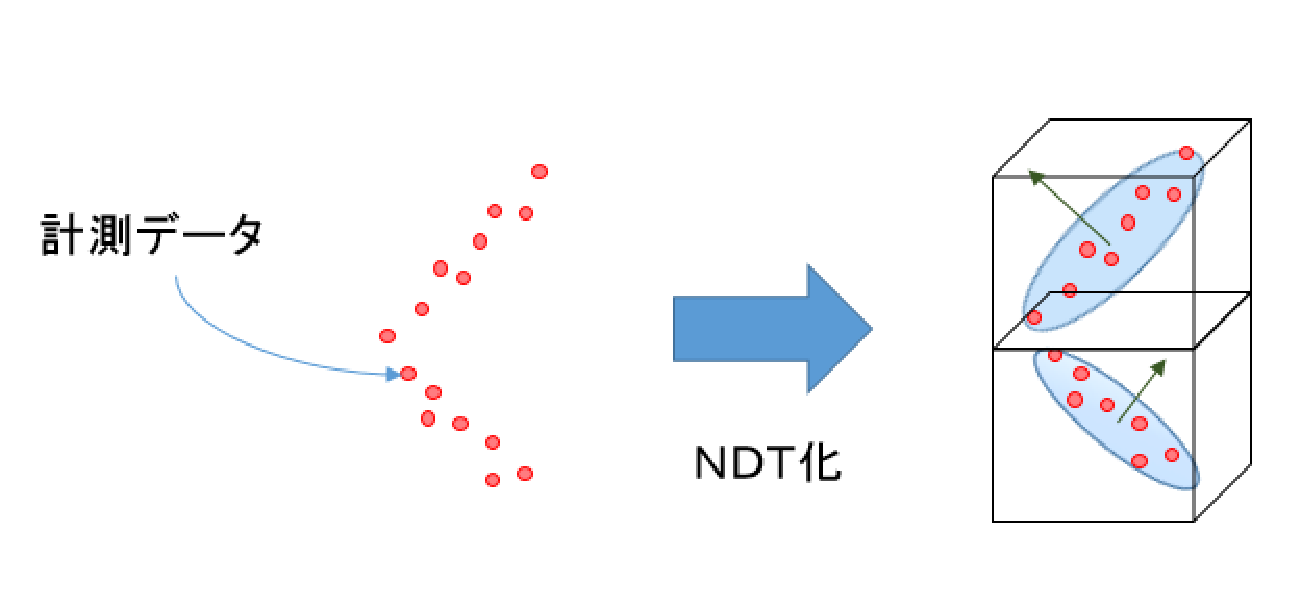
\includegraphics[height=55mm]{figure/NDTの概念.eps}
   \vspace{-5mm}
   \caption{NDTの概念}
   \label{NDTの概念}
  \end{center}
\end{figure}
%
\newpage
%
代表平面とは,各ボクセルにおいて,計算された3次元正規分布から分散値が最も小さい方向を法線ベクトルとする平面を言う.図2.1で説明すると,赤い点が計測された点群で,図2.1の右側にある格子がND ボクセル,また,青い楕円型が代表平面で緑色の矢印が代表平面の法線ベクトルである.\par
7つの代表点とは,得られた三次元正規分布に対して,各軸方向に半径$\sqrt{-2\ln \gamma}$の球面上の点を楕円上に射影した点6つと正規分布の中心点を合せた7つの点を言う.本研究では7つの代表点は計測データからのみにできるものとしている.つまり,地図データにはND ボクセルと代表平面,計測データにはND ボクセルと代表平面に加えて7つの代表点がある.データ構成を図{\ref{データ構成}}に表す.また,NDTにより得られる代表平面,代表点を図{\ref{NDTまとめ}}に表す.
%
\begin{figure}[htbp]
  \vspace{-3mm}
  \begin{center}
   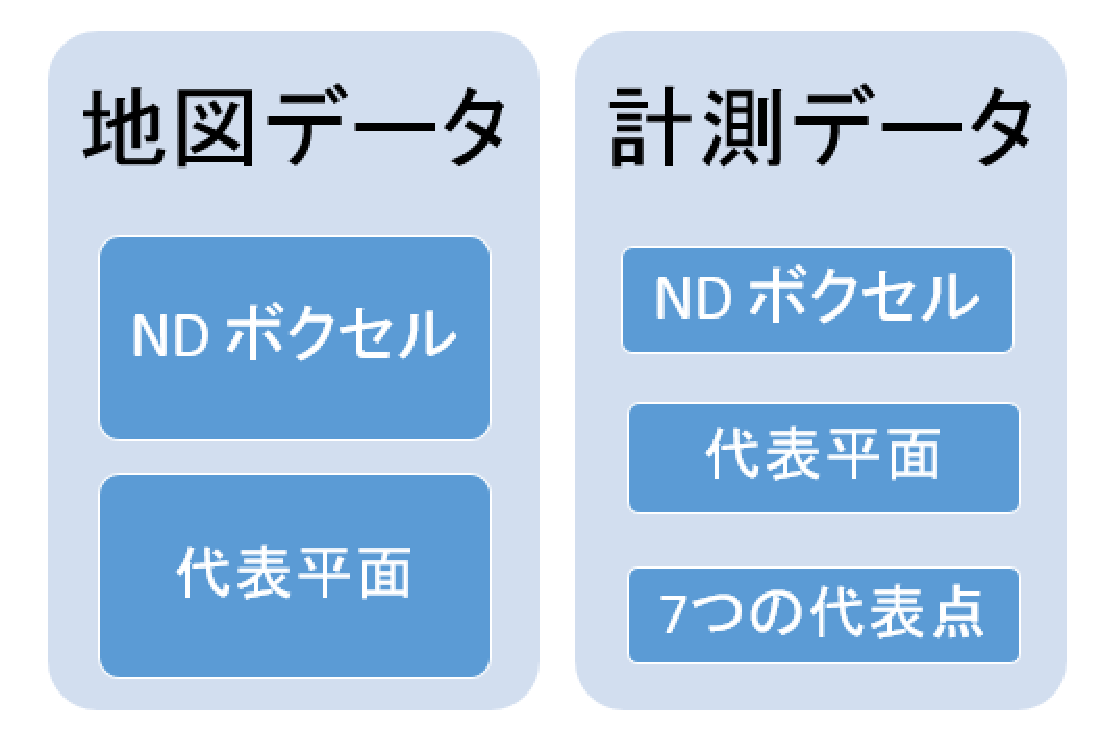
\includegraphics[height=55mm]{figure/データ構成.eps}
   \vspace{-5mm}
   \caption{データ構成}
   \label{データ構成}
  \end{center}
\end{figure}
%

%
\begin{figure}[htbp]
  \vspace{-3mm}
  \begin{center}
   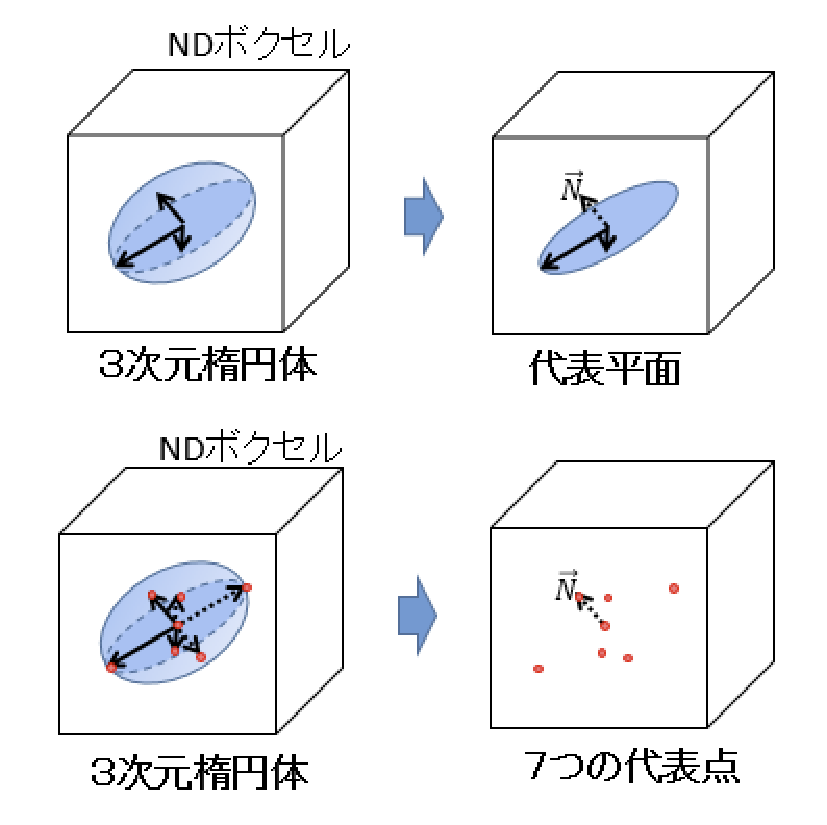
\includegraphics[height=65mm]{figure/NDTまとめ.eps}
   \vspace{-5mm}
   \caption{NDTまとめ}
   \label{NDTまとめ}
  \end{center}
\end{figure}
%

\newpage
%
しかし,NDTを利用してデータの簡略化はできるが,格子内に区切る離散化の影響により,境界付近に存在する点群形状が隣のボクセルで確認できないことがあり得る.対象ボクセルとその周りのすべてのボクセルとマッチング評価を行えば解決できるが,周りのすべてのボクセルは計27であるため,計算量が多くなるという問題がある.そこで,本研究では離散化の影響を低減するため,オーバーラップND ボクセルを用いる.オーバーラップND ボクセルとは,Biberら[3]の手法を3次元に拡張し,各格子を半分ずつ重複するようにし,1つの点が8つのボクセルに含まれるようにする手法である.図{\ref{オーバーラップNDボクセル}}にオーバーラップ NDボクセルの概念を表す.また,オーバーラップ NDボクセルの例を図{\ref{オーバーラップNDボクセルの例}}に表す.

%
\begin{figure}[htbp]
  \vspace{-3mm}
  \begin{center}
   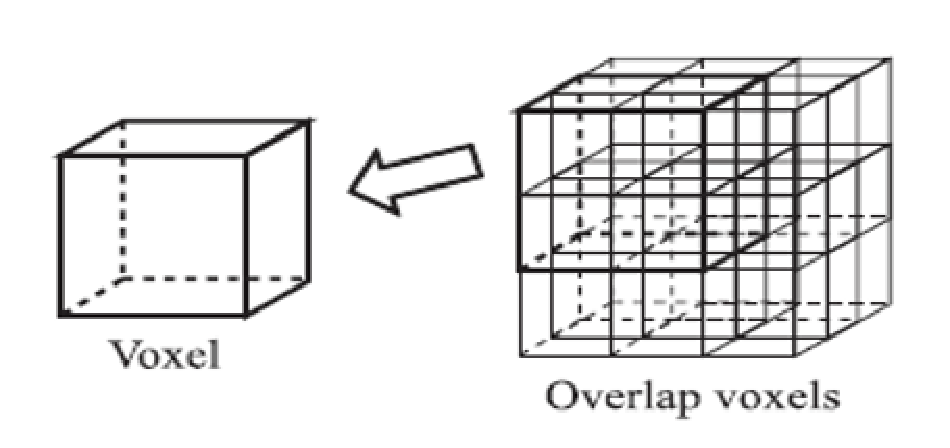
\includegraphics[height=55mm]{figure/オーバーラップNDボクセル.eps}
   \vspace{-5mm}
   \caption{オーバーラップNDボクセル([1]より引用)}
   \label{オーバーラップNDボクセル}
  \end{center}
\end{figure}
%
%
\begin{figure}[htbp]
  \vspace{-3mm}
  \begin{center}
   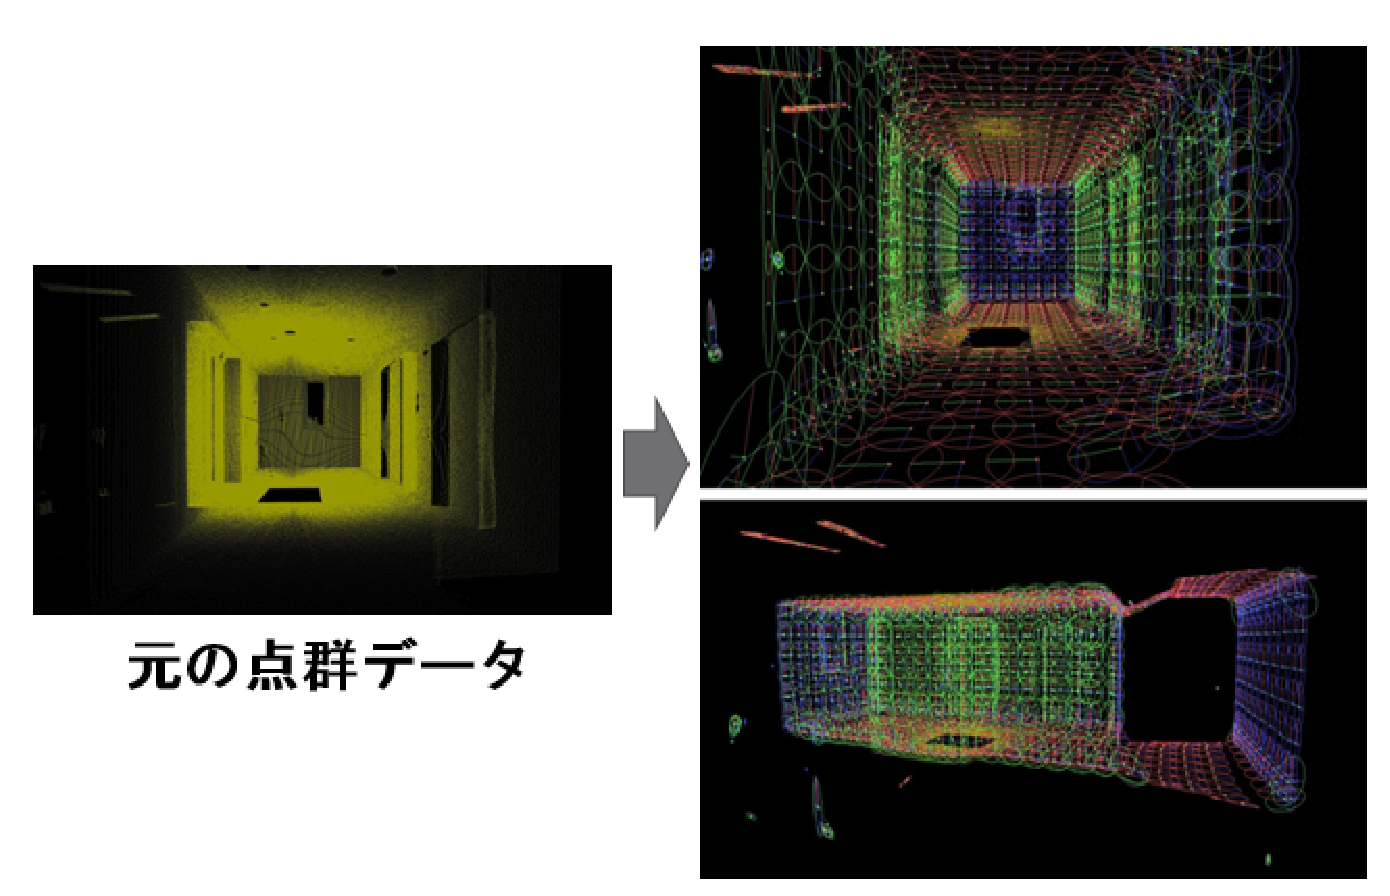
\includegraphics[height=55mm]{figure/オーバーラップNDボクセルの例.eps}
   \vspace{-5mm}
   \caption{オーバーラップNDボクセルの例([1]より引用)}
   \label{オーバーラップNDボクセルの例}
  \end{center}
\end{figure}
%
\newpage
%
NDTによりできるND ボクセルには大きさがあり,大きさを変えることでデータの解像度が変わる.ボクセルの大きさを小さくするほど,解像度は良くなるが,計算時間が増える.したがって,状況によってボクセルのサイズは変える必要がある.ボクセルのサイズによる解像度の例を図{\ref{ボクセルサイズによる解像度}}に表す.

\begin{figure}[htbp]
  \vspace{5mm}
  \begin{center}
   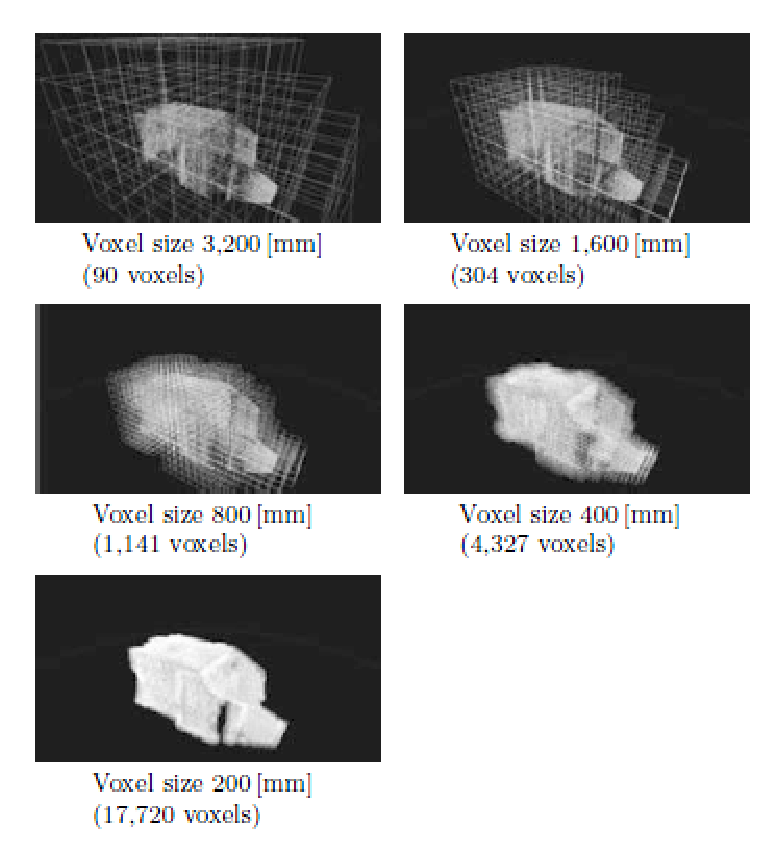
\includegraphics[height=120mm]{figure/ボクセルサイズによる解像度.eps}
   \vspace{-5mm}
   \caption{ボクセルサイズによる解像度([1]より引用)}
   \label{ボクセルサイズによる解像度}
  \end{center}
\end{figure}
%
\newpage
%
%---------------------------------------------------------------------------------------------------
\section{パーティクルフィルタ}
NDTにより3次元データの簡略化を行い,位置同定にはパーティクルフィルタを用いる.フィルタとは与えられた物から特定成分を取り除くまたは弱める作用をする機能を言う.ここで特定成分とはデータに含まれたノイズなどを含め,不確実性のデータをフィルタリングし正しい結果を推定することである.本研究ではパーティクルフィルタを用いて地図データの中から計測データと合致する位置を推定する.まずは,地図データ全体に決まった数のパーティクルをばら撒く.ばら撒いたパーティクルには重みと状態量があって、最初の位置から次の位置まで移動量を予測する.その次に前状態の情報を用いて移動方向に対して尤度(もっともらしい値)を計算する.そこで,ある基準からパーティクル尤度の値が低かったら,そのパーティクルは削減される.またパーティクル尤度の値が大きいほど,その周りにはパーティクルが集中するようになる.集中されたパーティクルを用いて同じ過程を繰り返し,最終的に収束される位置が推定する位置となる.本研究のパーティクルフィルタの流れを簡単にまとめる.
\begin{enumerate}
\item 初期化:パーティクルを位置・姿勢地図データ全体にランダムにばら撒く.4に進む.
\item リサンプリング:以前時刻のパーティクルのうち一つのその重みを確率としてランダムに選択し,指定された最大パーティクル数分繰り返し選択する.
\item 予測:選択された各々のパーティクルに対してシステムの動作モデルを適用し,現時刻のシステムの状態(位置・姿勢)を予測する.
\item 尤度計算,重み付け:測定情報と各々のパーティクルの状態から評価関数によって尤度計算を行い,その結果を新たな重みと付ける.
\item 2に戻る.
\end{enumerate}

\newpage
%
%---------------------------------------------------------------------------------------------------
\section{地図データと計測データとのマッチング(尤度計算)}
ND ボクセルで表された地図データと計測データを用いて,パーティクルフィルタにより位置追跡を行う.各パーティクルには各々候補となるロボットの位置t,姿勢Rを持つ.尤度計算手順の流れを図{\ref{尤度計算手順}}に表す.\par

\vspace{10mm}
\begin{figure}[htbp]
  \begin{center}
   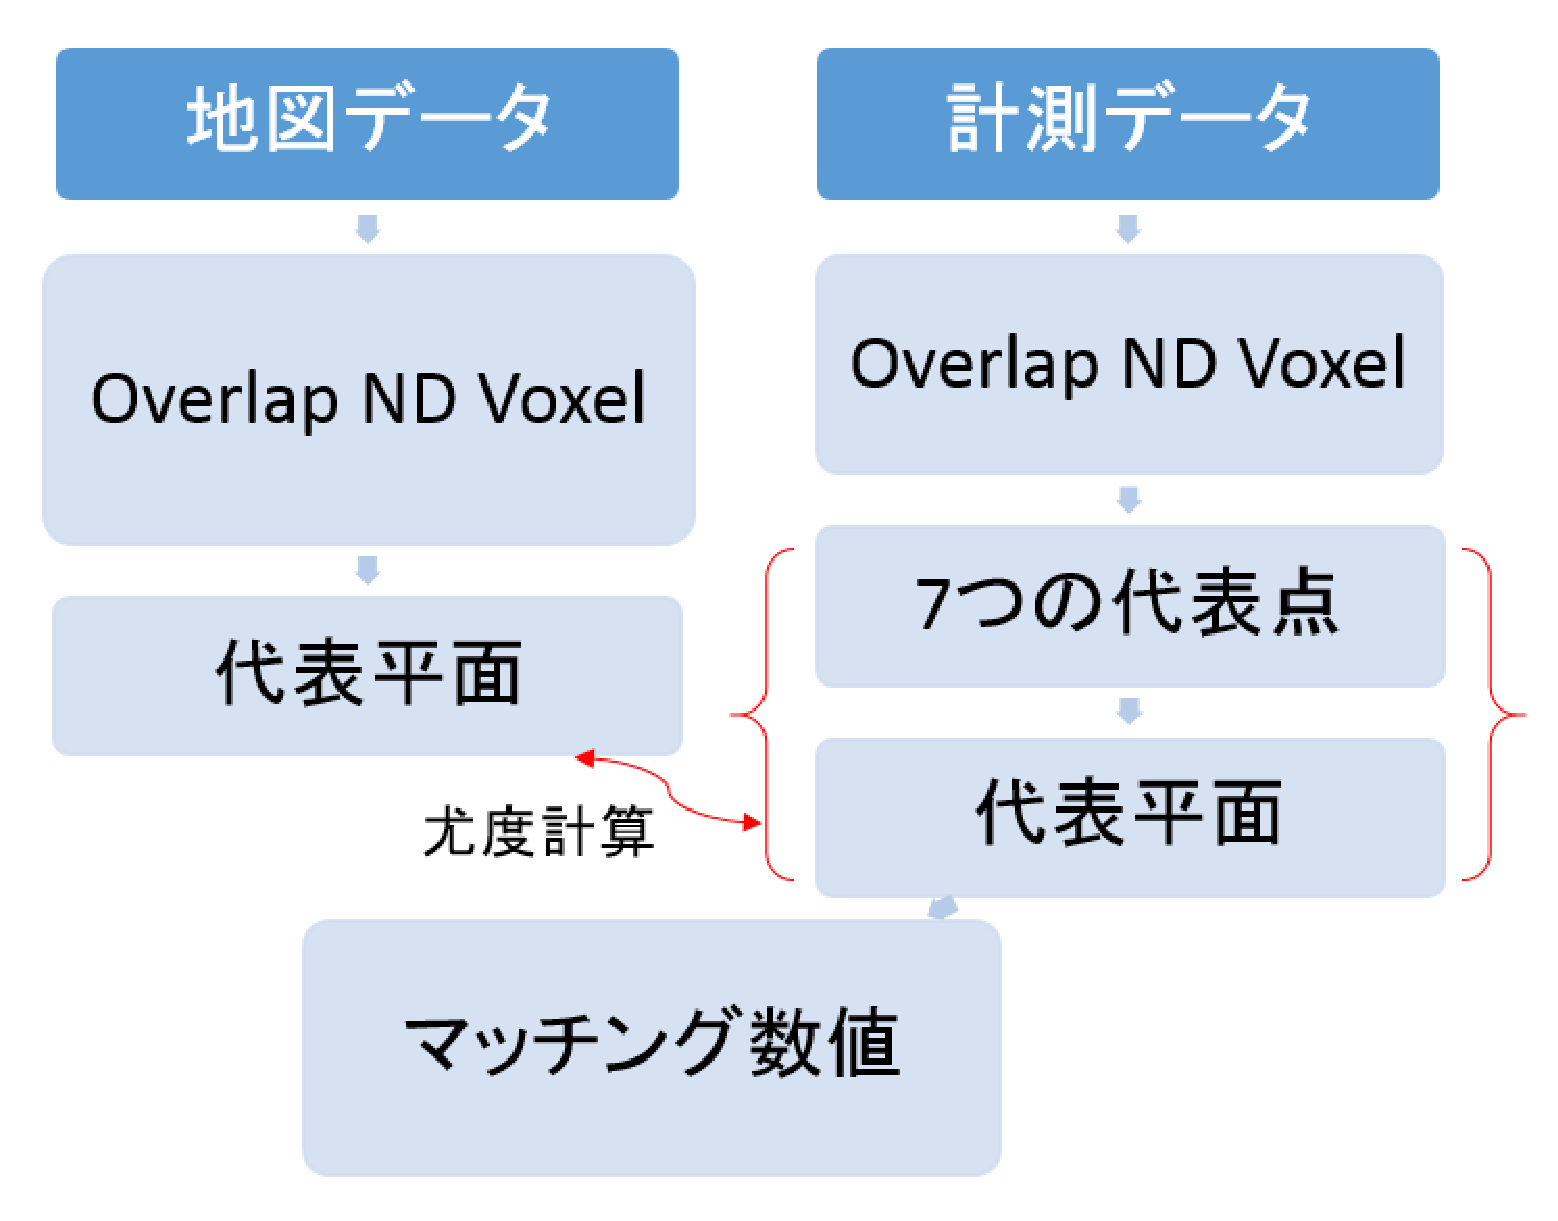
\includegraphics[height=70mm]{figure/尤度計算手順.eps}
   \caption{尤度計算手順}
   \label{尤度計算手順}
  \end{center}
\end{figure}
%
まず,計測データ中の各ボクセルを位置姿勢候補で座標変換し,地図データの各ボクセル中の代表平面と計測データの代表点との距離及び代表平面の法線の角度差を計算する.計算データのボクセルiにおける代表点k(k = 1~7)を$S_{ik}$ = $(S_{ikx},S_{iky},S_{ikz})^T$とし,代表平面の法線ベクトルを$N_{i}$ = $(N_{ix},N_{iy},N_{iz})^T$とすると,位置姿勢変換後の代表点$\tilde{S}_{ik}$,代表平面の法線ベクトル$\tilde{N}_{i}$は以下のようになる.また,図{\ref{尤度計算}}に尤度計算の概念を表す.

\begin{equation}
\tilde{S}_{ik} = RS_{ik} + t
\end{equation}
\begin{equation}
\tilde{N}_{i} = RN_{i}
\end{equation}

\vspace{5mm}
\begin{figure}[htbp]
  \begin{center}
   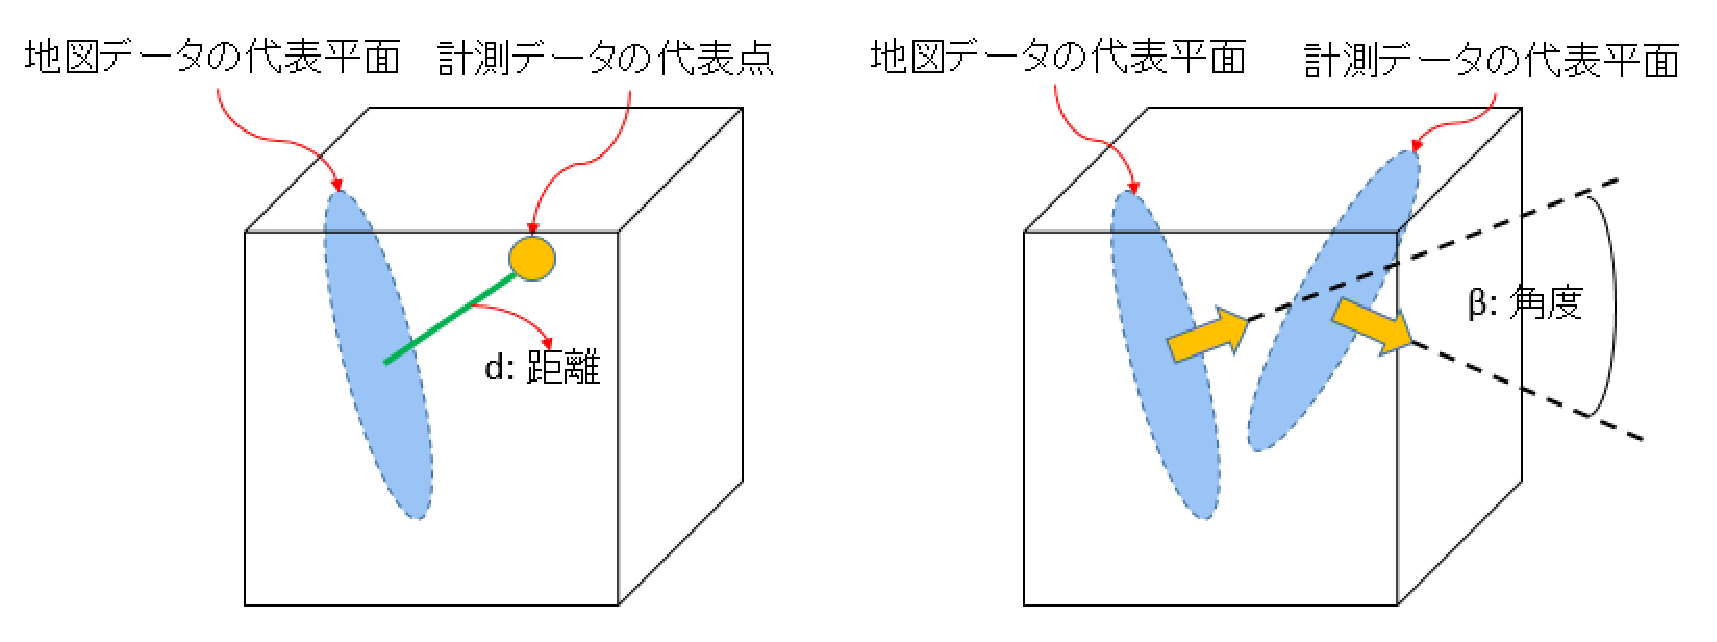
\includegraphics[height=60mm]{figure/尤度計算.eps}
   \caption{尤度計算}
   \label{尤度計算}
  \end{center}
\end{figure}
%
\vspace{15mm}
位置姿勢変換後の代表点が含まれる地図データ中の8個のオーバーラップ化されたボクセルm (m = 1~8)に対し,計測データの代表点と地図データの代表平面との距離$d_{ik->m}$を求める.正規分布に当てはめた代表点$\tilde{S}_{ik}$の距離評価値を$\alpha_{ik->m}$とする.地図データ中のボクセルmにおける代表平面の法線ベクトルを$N_{m}$とし,地図データ中のボクセルmの点群の平均位置を$\mu_{m}$とおくと,距離$d_{ik->m}$,$\alpha_{ik->m}$は以下のようになる.ここで$\sigma_{d}$は$d_{ik->m}$の分散値を表すパラメータである.図{\ref{尤度計算}}の左図に相当する計算である.\par

\begin{equation}
d_{ik->m} = |N_{mx}(S_{ikx}-\mu_{mx})+N_{my}(S_{iky}-\mu_{my})+N_{mz}(S_{ikz}-\mu_{mz})|
\end{equation}
\begin{equation}
\alpha_{ik->m} = \cfrac{1}{\sqrt{2\pi\sigma_{d}}}e^{-d^2_{ik->m}/\sigma_{d}^2}
\end{equation}

地図データのボクセルmと計測データのボクセルiの代表平面の相対角度の差を評価値$\beta_{i->m}$とする.$\beta_{i->m}$は以下のように求める.図{\ref{尤度計算}}から言うと右図に相当する計算である.\par
\begin{equation}
\beta_{i->m} = |N_{mx}\tilde{N}_{ix}+N_{my}\tilde{N}_{iy}+N_{mz}\tilde{N}_{iz}|
\end{equation}

代表点$S_{ik}$の総合評価値$\gamma_{ik}$は距離評価値を$\alpha_{ik->m}$と相対角度評価値$\beta_{i->m}$の積で求められるが,オーバーラップ化されている場合は以下のように各々の8つのボクセルで求めた総合評価値$\gamma_{ik}$の最大値として求める.\par

\begin{equation}
\gamma_{ik} = \max_{1 \leq m \leq 8}\alpha_{ik->m}\beta_{i->m}
\end{equation}

計測データボクセルiの評価値$\delta_{i}$はボクセルiにおける7つの代表点に対して評価値の和を計算する.最後に,計測データの全てのボクセル数に対して,評価値$\delta_{i}$の値を足すとパーティクルスコア$\lambda$が求められる.式は以下のようになる.\par

\begin{equation}
\delta_{i} = \sum_{k=1}^{7}\gamma_{ik}
\end{equation}

\begin{equation}
\lambda = \sum_{i=1}^{N}\delta_{i}
\end{equation}

まとめると,式(2.5)から(2.7)までは距離評価値を$\alpha_{ik->m}$と相対角度評価値$\beta_{i->m}$をもとめ,それらの値の積で,計測された代表点$\S_{ik}$の総合評価値$\gamma_{ik}$を計算している.これはそれぞれの評価値を条件付き確率とみなし,代表点ごとの尤度を計算したものである.式(2.9)と式(2.10)は式(2.5)から(2.7)の尤度計算で求めた各代表点の評価値を全代表点及び全ボクセルの数分足したものである.最後に求められたパーティクルスコア$\lambda$が最終的な重さとなる.


\newpage
パーティクルフィルタを用いて収束する過程の例を図{\ref{収束過程の例}}に表す.図2.9で,緑はパーティクルの位置,青は3次元地図,赤は計測した3次元点,黒は最も尤度が高いパーティクルの位置である.
\vspace{10mm}
\begin{figure}[htbp]
  \begin{center}
   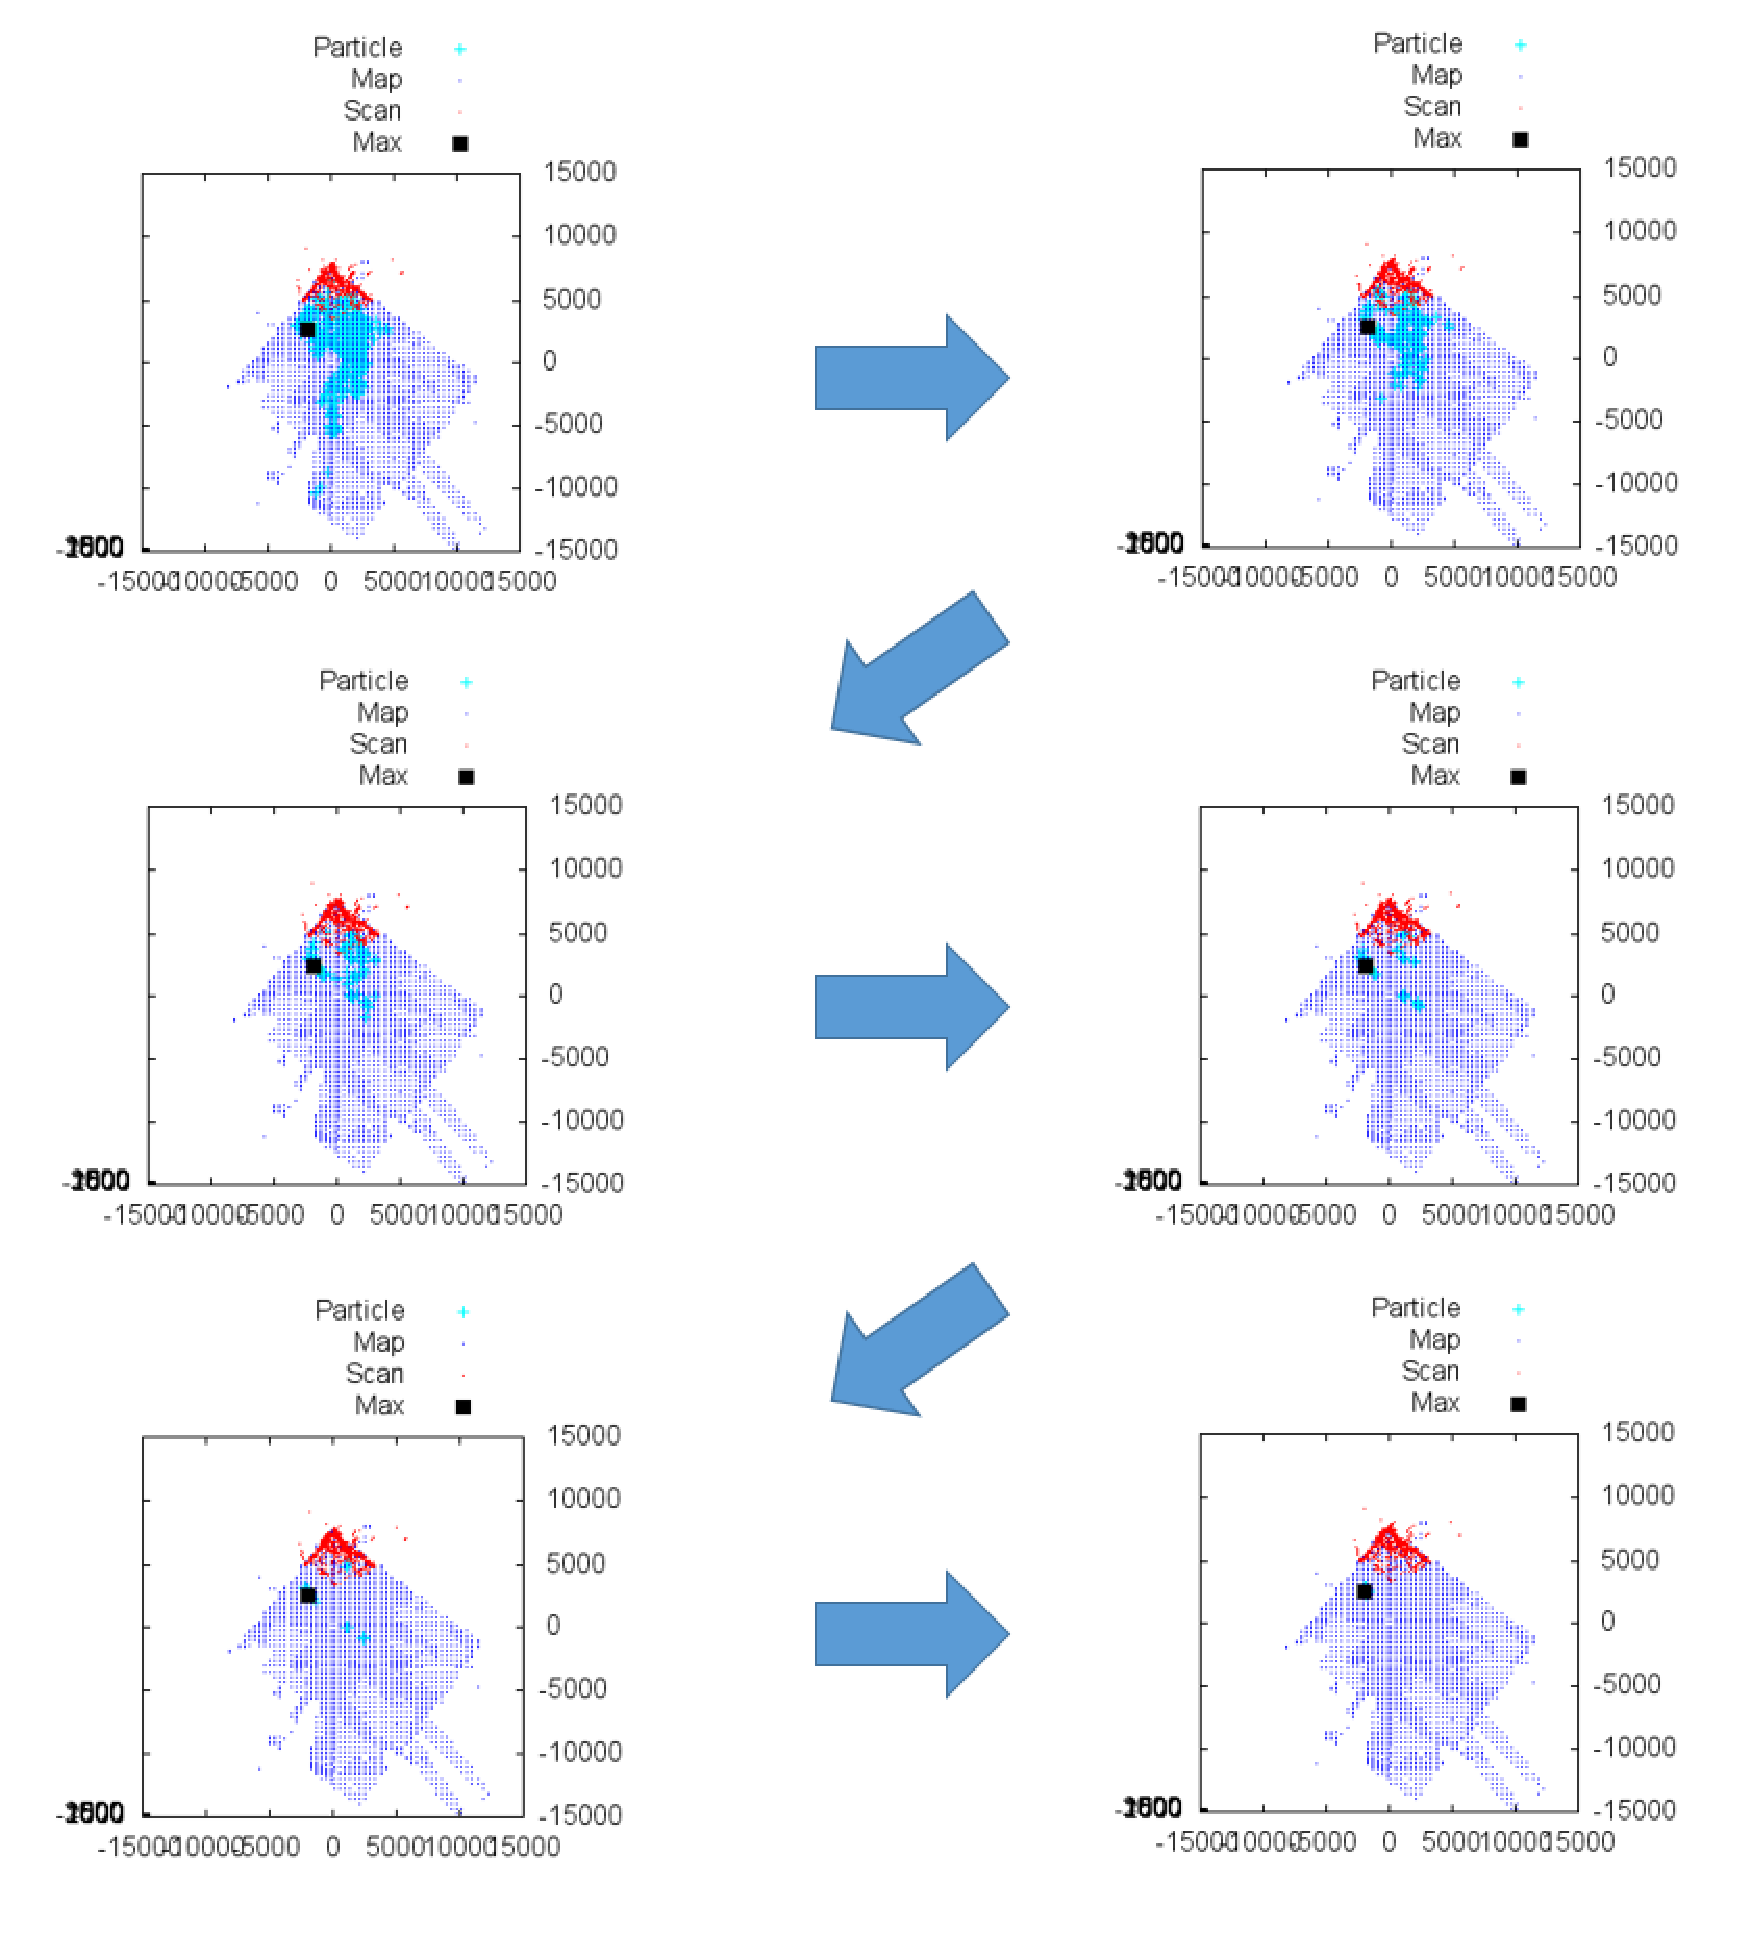
\includegraphics[height=150mm]{figure/収束過程の例.eps}
   \caption{収束過程の例}
   \label{収束過程の例}
  \end{center}
\end{figure}
%
\newpage
%
%---------------------------------------------------------------------------------------------------